\chapter{Urban Source Identification Results and Discussion}

% Compare how well we identify shielded/unshielded isotopes when training set has shielding, doesn't have shielding. 

% Compare how well we identify isotopes over different distances if training set has one vs many distances

% Compare how well we identify isotopes with different calibration sampling granularity 

% https://e-reports-ext.llnl.gov/pdf/312592.pdf holy shit they show common false positive isotopes and we see a lot of overlap



\section{Problem Description and Training Dataset Overview}

This chapter applies machine learning algorithms to solve the problem of identifying a radioactive source in an urban environment where a source may be present. This scenario is applicable when performing source interdiction searching cargo containers, vehicles at boarder crossings, or security at high profile events. Urban environments present unique challenges to gamma-ray spectroscopy. Background radiation can change over city blocks due to different concentrations of uranium and thorium in building materials. Sources may be purposely shielded by unknown amounts of material to obscure their gamma-ray signal.





\section{Data Augmentation Implementation}

Because simulating a dataset with sufficient combinations of available data augmentation - seen in Tables \ref{table:all_fixed_simulation_parameters} and \ref{table:all_variable_simulation_parameters} - online data augmentation techniques are employed. Online data augmentation has the benefit of implicitly regularizing the models.

Steps in the data augmentation process are:
\begin{enumerate}
  \item Randomly choose a background template with the same FWHM as the source template
  \item Rebin source and background template with a random calibration
  \item Apply the LLD to both templates
  \item Normalize both templates by the sum of their respective counts 
  \item Scale both signals by their respective total counts
  \begin{itemize}
     \item Counts defined by randomly chosen background counts per second, integration time, and signal to background ratio
   \end{itemize}
  \item Add both signals 
  \item Poisson sample the resulting signal
\end{enumerate}


\section{Learning Curve Comparison for Fixed-size Datasets and Online Data Augmentation Datasets}

In this section we use learning curves to quantify how well the online data augmentation improved testing error. Learning curves are [definition, explanation]. Learning curves are used to determine a few things. We will use them to do [the following].

First, They are used as a sanity check, to make sure we are sampling our input space with enough granularity. To know we are sampling well enough, we should be sampling in a region where the curves are flat for both algorithms.

Secondly, Learning curves give us insight into which algorithm works better on the hyperparameter optimization dataset and simplified version of the problem. We're expecting the CNN to outperform the DNN due to theoretical benefits of convolution architectures for our problem. We can also compare this curve to the final learning curves for the final datasets.

For the autoencoders, pretraining was done using a fixed dataset of 10000 samples. Because of the implicit regularization of the undercomplete encoding and the denoising background subtracting process, both networks do not use a additional regularization when training. The initial learning rate of each autoencoder was set to 10$^{-5}$.


\begin{figure}[H]
	\centering
	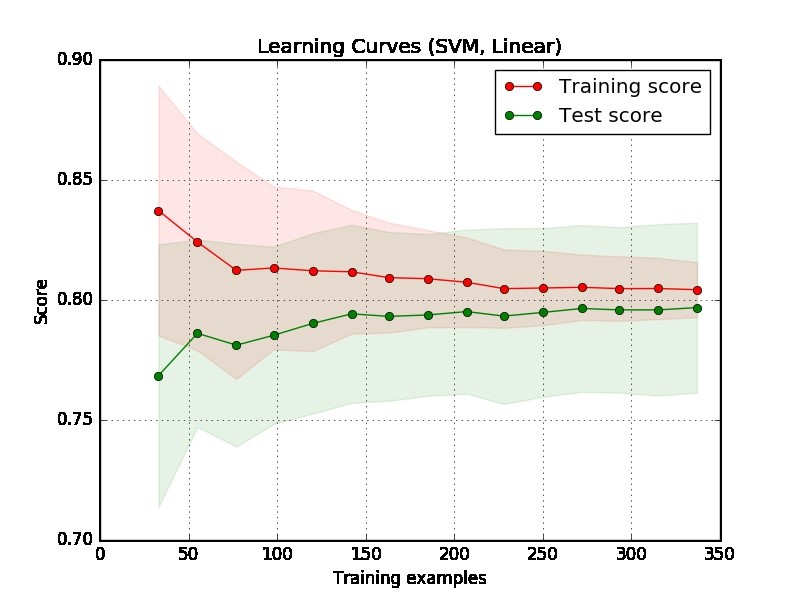
\includegraphics[width=0.8\linewidth]{model_choice_hyperparameter_search_images/learning_curve_dummy}
	\caption{Learning curves from the best DNN with best performance from online data augmentation. Shown: learning curve example.}
	\label{fig:learning_curves}
\end{figure}



\begin{figure}[H]
	\centering
	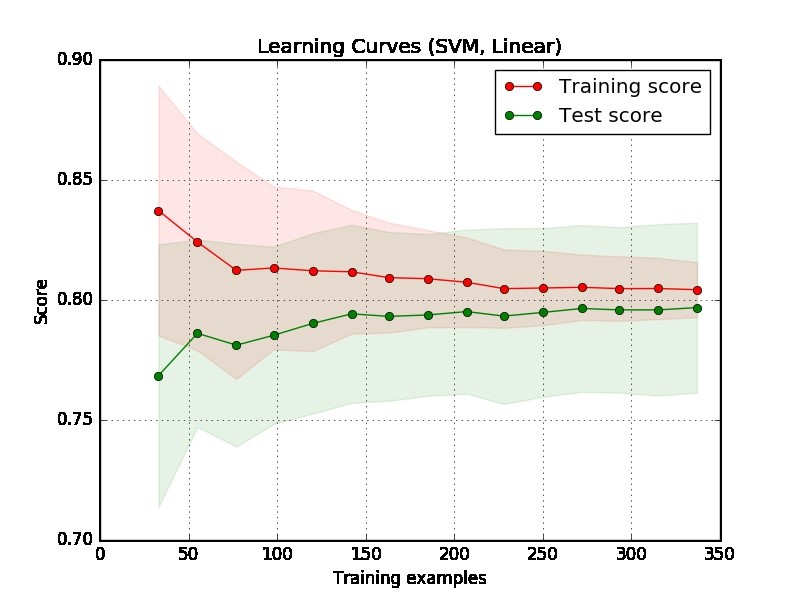
\includegraphics[width=0.8\linewidth]{model_choice_hyperparameter_search_images/learning_curve_dummy}
	\caption{Learning curves from the best CNN with best performance from online data augmentation. Shown: learning curve example.}
	\label{fig:learning_curves}
\end{figure}


\section{Generalization Performance Evaluation}

In this section we analyze the generalization performance of each network and training dataset. To quantify performance on a range of spectra qualities, the F1-scores for each bagged model are shown over integration time and signal to background ratios of 0.1 and 0.5.

% When the error between models differs significantly or is particularly large, confusion matrices are included to show what isotopes are problematic.

\subsection{Generalization Performance on Source-Detector Distance and Height Off Ground}

In this section we analyze the generalization performance of each network on changes in source-detector distance and height. This tests if each model is sensitive to changes in the Compton continuum due to environmental scattering. Good performance in these simulated data may indicate better performance in real data.

To test generalization performance, datasets are simulated with unshieled spectral templates with a FWHM of 7.5. 


\begin{figure}[H]
     \centering
     \begin{subfigure}[b]{0.49\textwidth}
         \centering
         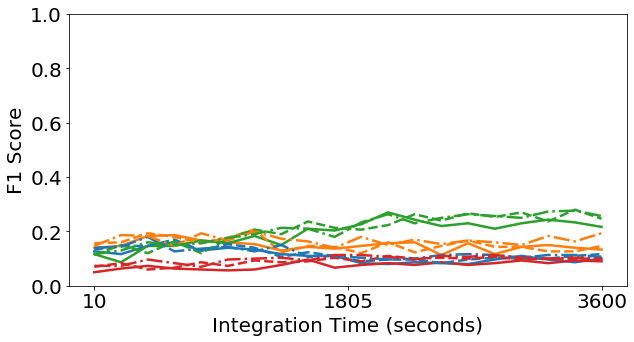
\includegraphics[width=\textwidth]{images/generalization-height-easy-01.png}
         \caption{}
         \label{fig:generalization-height-easy-01}
     \end{subfigure}
     \hfill
     \begin{subfigure}[b]{0.49\textwidth}
         \centering
         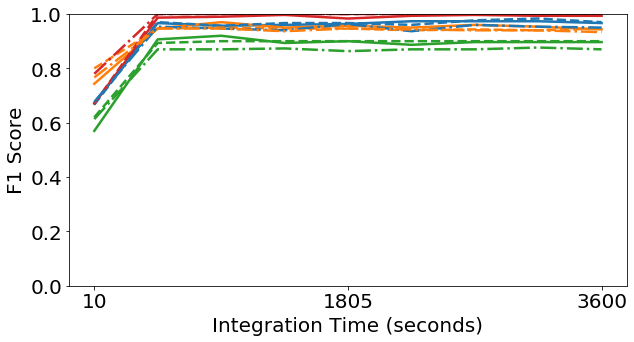
\includegraphics[width=\textwidth]{images/generalization-height-easy-05.png}
         \caption{}
         \label{fig:generalization-height-easy-05}
     \end{subfigure}

     \begin{subfigure}[b]{0.49\textwidth}
         \centering
         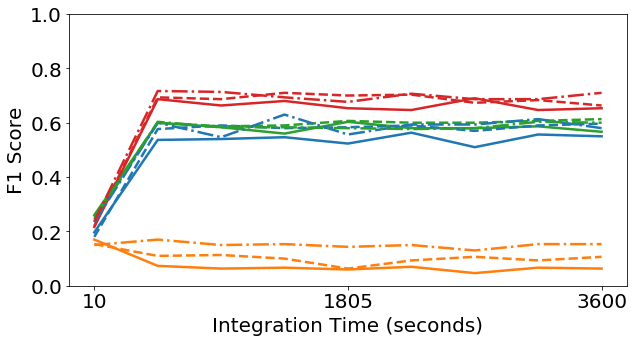
\includegraphics[width=\textwidth]{images/generalization-height-full-01.png}
         \caption{}
         \label{fig:generalization-height-full-01}
     \end{subfigure}
     \hfill
     \begin{subfigure}[b]{0.49\textwidth}
         \centering
         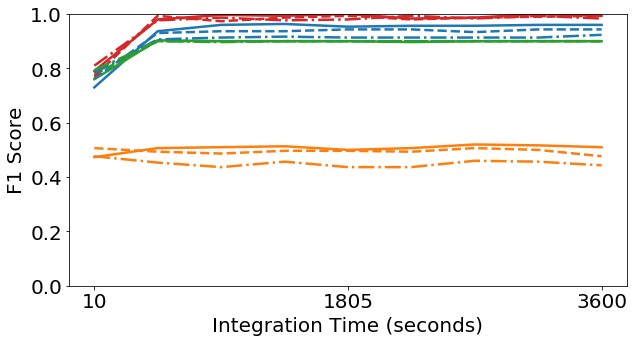
\includegraphics[width=\textwidth]{images/generalization-height-full-05.png}
         \caption{}
         \label{fig:generalization-height-full-05}
     \end{subfigure}

        \caption{Height-off-ground generalization performance of the DNN, CNN with and without autoencoder pretraining. F1 score shown in averaged over five networks trained with 10000 total dataset examples,}
        \label{fig:generalization_height_fixeddataset}
\end{figure}



\begin{figure}[H]
     \centering
     \begin{subfigure}[b]{0.49\textwidth}
         \centering
         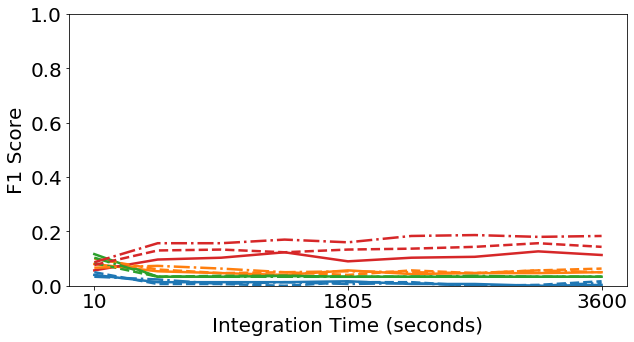
\includegraphics[width=\textwidth]{images/generalization-height-aug-easy-01.png}
         \caption{}
         \label{fig:generalization-height-aug-easy-01}
     \end{subfigure}
     \hfill
     \begin{subfigure}[b]{0.49\textwidth}
         \centering
         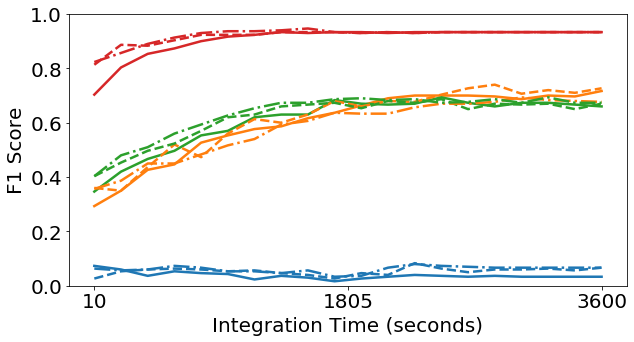
\includegraphics[width=\textwidth]{images/generalization-height-aug-easy-05.png}
         \caption{}
         \label{fig:generalization-height-aug-easy-05}
     \end{subfigure}

     \begin{subfigure}[b]{0.49\textwidth}
         \centering
         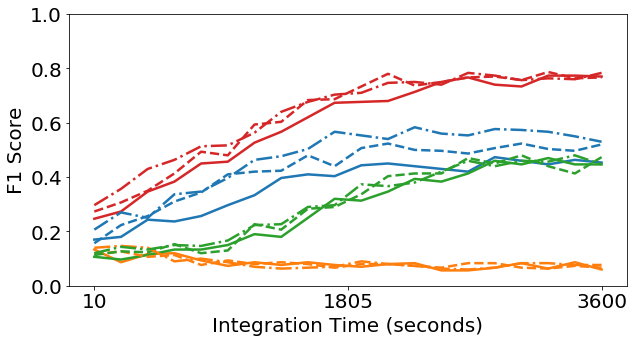
\includegraphics[width=\textwidth]{images/generalization-height-aug-full-01.png}
         \caption{}
         \label{fig:generalization-height-aug-full-01}
     \end{subfigure}
     \hfill
     \begin{subfigure}[b]{0.49\textwidth}
         \centering
         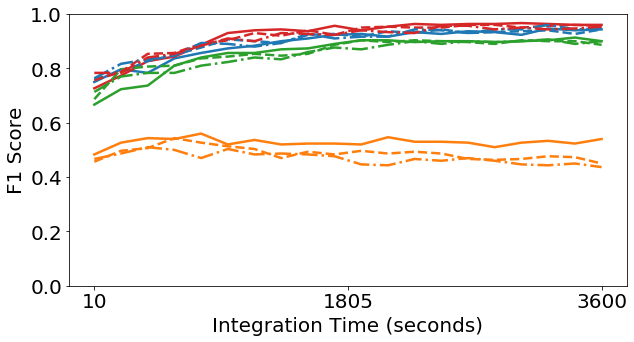
\includegraphics[width=\textwidth]{images/generalization-height-aug-full-05.png}
         \caption{}
         \label{fig:generalization-height-aug-full-05}
     \end{subfigure}

        \caption{Height-off-ground generalization performance of the DNN, CNN with and without autoencoder pretraining. F1 score shown in averaged over five networks trained with data augmentation,}
        \label{fig:generalization_height_augdataset}
\end{figure}

\subsection{Generalization Performance on Source-Detector Standoff Distance}


\begin{figure}[H]
     \centering
     \begin{subfigure}[b]{0.49\textwidth}
         \centering
         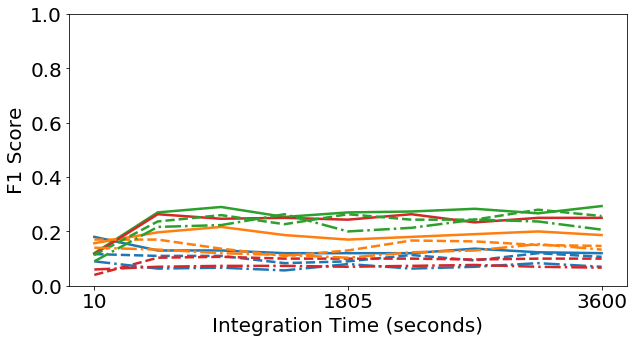
\includegraphics[width=\textwidth]{images/generalization-dist-easy-01.png}
         \caption{}
         \label{fig:generalization-dist-easy-01}
     \end{subfigure}
     \hfill
     \begin{subfigure}[b]{0.49\textwidth}
         \centering
         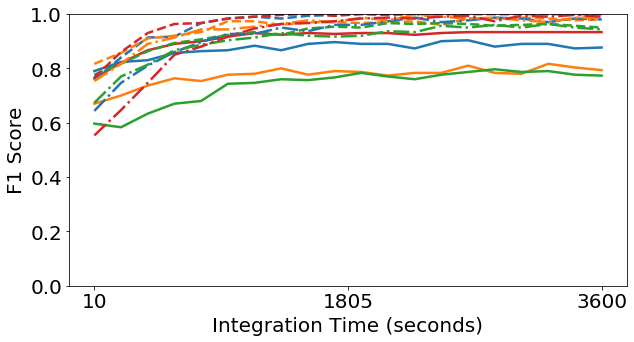
\includegraphics[width=\textwidth]{images/generalization-dist-easy-05.png}
         \caption{}
         \label{fig:generalization-dist-easy-05}
     \end{subfigure}

     \begin{subfigure}[b]{0.49\textwidth}
         \centering
         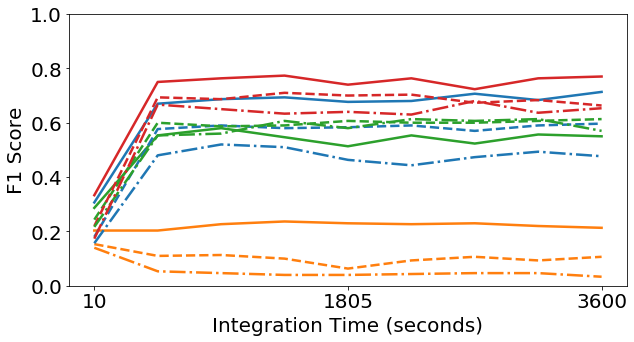
\includegraphics[width=\textwidth]{images/generalization-dist-full-01.png}
         \caption{}
         \label{fig:generalization-dist-full-01}
     \end{subfigure}
     \hfill
     \begin{subfigure}[b]{0.49\textwidth}
         \centering
         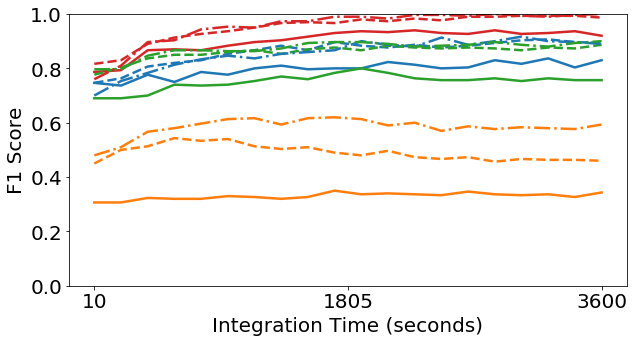
\includegraphics[width=\textwidth]{images/generalization-dist-full-05.png}
         \caption{}
         \label{fig:generalization-dist-full-05}
     \end{subfigure}

        \caption{Standoff distance generalization performance of the DNN, CNN with and without autoencoder pretraining. F1 score shown in averaged over five networks trained with 10000 total dataset examples,}
        \label{fig:generalization_distt_fixeddataset}
\end{figure}




\begin{figure}[H]
     \centering
     \begin{subfigure}[b]{0.49\textwidth}
         \centering
         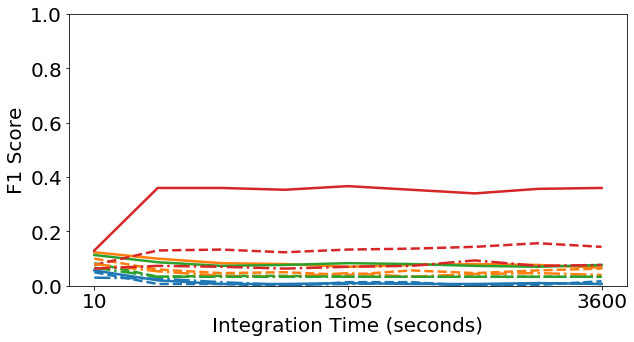
\includegraphics[width=\textwidth]{images/generalization-dist-aug-easy-01.png}
         \caption{}
         \label{fig:generalization-dist-aug-easy-01}
     \end{subfigure}
     \hfill
     \begin{subfigure}[b]{0.49\textwidth}
         \centering
         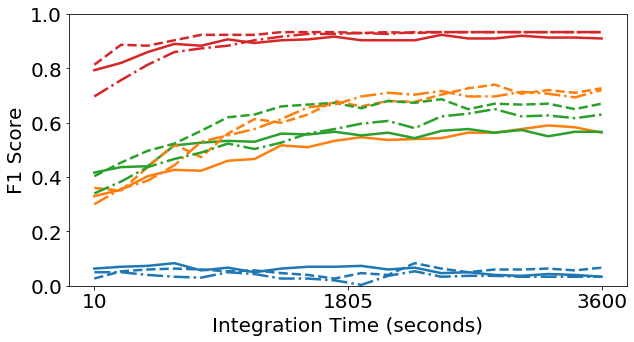
\includegraphics[width=\textwidth]{images/generalization-dist-aug-easy-05.png}
         \caption{}
         \label{fig:generalization-dist-aug-easy-05}
     \end{subfigure}

     \begin{subfigure}[b]{0.49\textwidth}
         \centering
         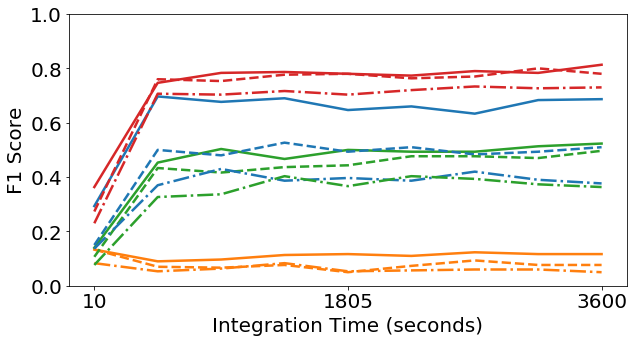
\includegraphics[width=\textwidth]{images/generalization-dist-aug-full-01.png}
         \caption{}
         \label{fig:generalization-dist-aug-full-01}
     \end{subfigure}
     \hfill
     \begin{subfigure}[b]{0.49\textwidth}
         \centering
         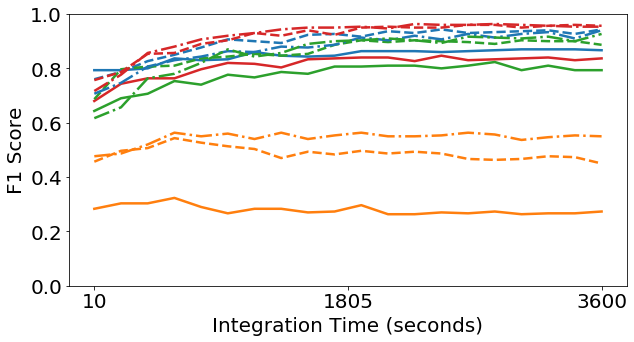
\includegraphics[width=\textwidth]{images/generalization-dist-aug-full-05.png}
         \caption{}
         \label{fig:generalization-dist-aug-full-05}
     \end{subfigure}

        \caption{Standoff distance generalization performance of the DNN, CNN with and without autoencoder pretraining. F1 score shown in averaged over five networks trained with data augmentation,}
        \label{fig:generalization_dist_augdataset}
\end{figure}



\subsection{Generalization Dependence on Full-Width-at-Half-Max}


\subsection{Generalization Dependence on Shielding.}

Datasets were simulated with and without shielding. 





\subsection{Generalization Dependence on Calibration.}

Datasets were simulated with various gain and offset setting.


\begin{figure}[H]
     \centering
     \begin{subfigure}[b]{0.49\textwidth}
         \centering
         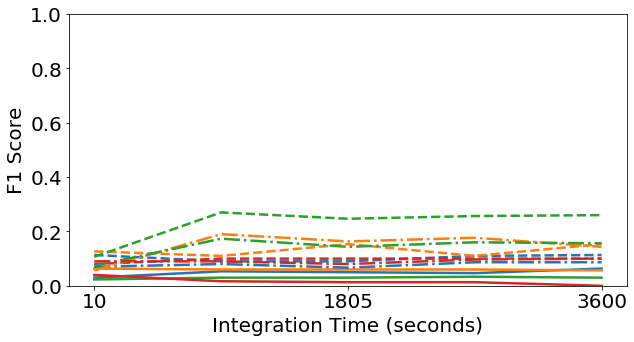
\includegraphics[width=\textwidth]{images/generalization-cal-easy-01.png}
         \caption{}
         \label{fig:generalization-dist-easy-01}
     \end{subfigure}
     \hfill
     \begin{subfigure}[b]{0.49\textwidth}
         \centering
         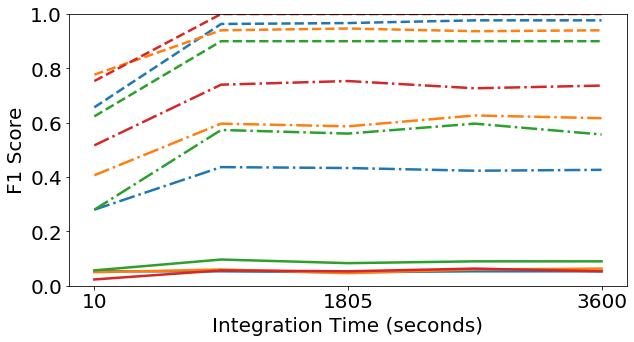
\includegraphics[width=\textwidth]{images/generalization-cal-easy-05.png}
         \caption{}
         \label{fig:generalization-dist-easy-05}
     \end{subfigure}

     \begin{subfigure}[b]{0.49\textwidth}
         \centering
         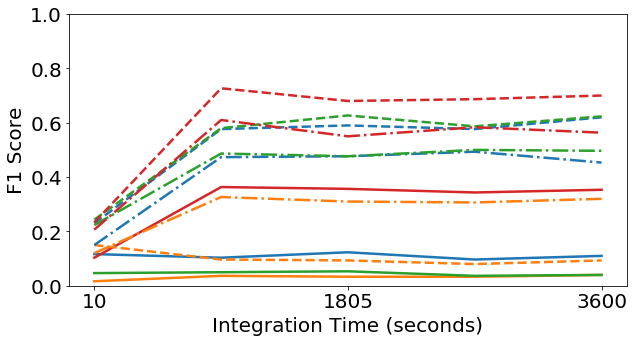
\includegraphics[width=\textwidth]{images/generalization-cal-full-01.png}
         \caption{}
         \label{fig:generalization-dist-full-01}
     \end{subfigure}
     \hfill
     \begin{subfigure}[b]{0.49\textwidth}
         \centering
         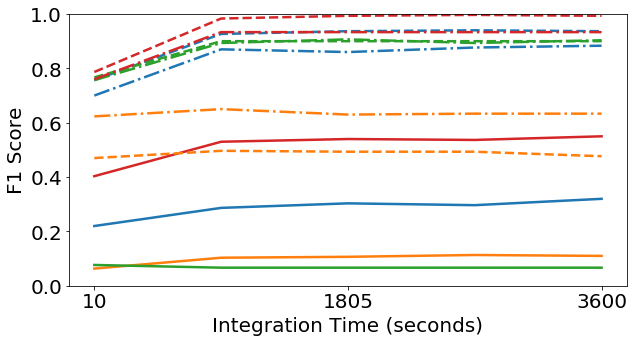
\includegraphics[width=\textwidth]{images/generalization-cal-full-05.png}
         \caption{}
         \label{fig:generalization-dist-full-05}
     \end{subfigure}

        \caption{Calibration gain generalization performance of the DNN, CNN with and without autoencoder pretraining. F1 score shown in averaged over five networks trained with 10000 total dataset examples,}
        \label{fig:generalization_distt_fixeddataset}
\end{figure}




\begin{figure}[H]
     \centering
     \begin{subfigure}[b]{0.49\textwidth}
         \centering
         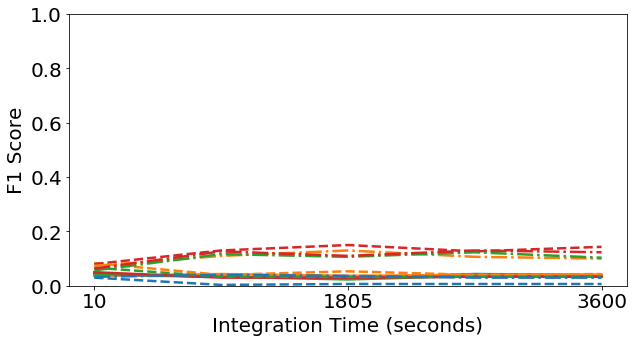
\includegraphics[width=\textwidth]{images/generalization-cal-aug-easy-01.png}
         \caption{}
         \label{fig:generalization-dist-aug-easy-01}
     \end{subfigure}
     \hfill
     \begin{subfigure}[b]{0.49\textwidth}
         \centering
         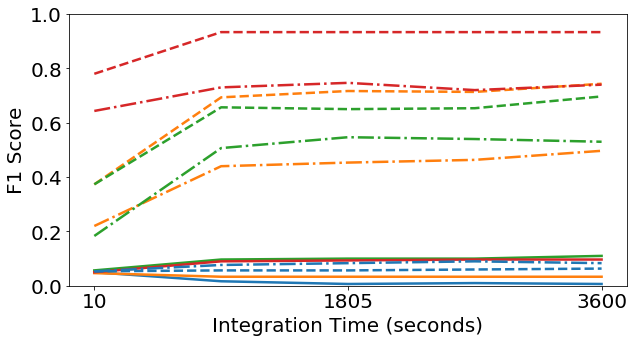
\includegraphics[width=\textwidth]{images/generalization-cal-aug-easy-05.png}
         \caption{}
         \label{fig:generalization-dist-aug-easy-05}
     \end{subfigure}

     \begin{subfigure}[b]{0.49\textwidth}
         \centering
         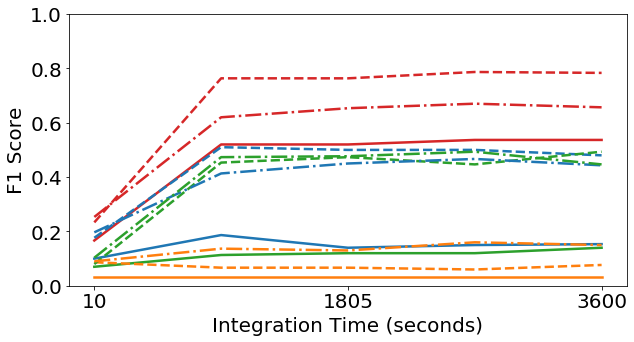
\includegraphics[width=\textwidth]{images/generalization-cal-aug-full-01.png}
         \caption{}
         \label{fig:generalization-dist-aug-full-01}
     \end{subfigure}
     \hfill
     \begin{subfigure}[b]{0.49\textwidth}
         \centering
         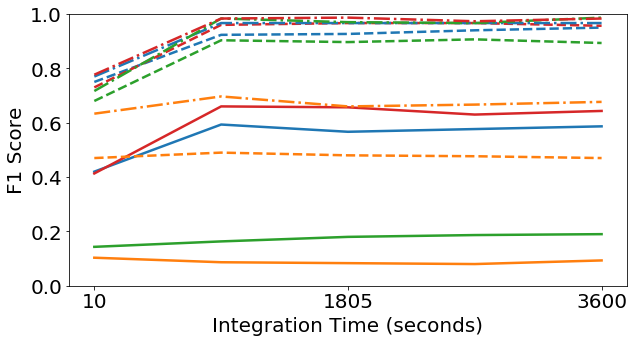
\includegraphics[width=\textwidth]{images/generalization-cal-aug-full-05.png}
         \caption{}
         \label{fig:generalization-dist-aug-full-05}
     \end{subfigure}

        \caption{Calibration gain generalization performance of the DNN, CNN with and without autoencoder pretraining. F1 score shown in averaged over five networks trained with data augmentation,}
        \label{fig:generalization_dist_augdataset}
\end{figure}

% \subsection{Generalization Dependence on Changing Background.}

% Datasets were simulated with backgrounds different from the training set and real measured background. It is expected that the complete dataset will mistake background for isotopes more often than the simplified dataset because photopeaks are decreased by shielding.


\subsection{Results on Spectra for ANSI compliance}

This section shows model asymptotic performance vs integration time for ANSI compliance. Using N models (justified previously as asymptotic). 



\begin{table}[H]
\centering
\caption{Isotope combinations required for the ANSI standard \cite{ANSI}.}
\begin{tabular}{c}
Isotope Combinations \\ \hline
$^{137}$Cs + depleted uranium (DU) \\ % \hline
$^{99m}$Tc + HEU \\ % \hline
$^{201}$Tl + HEU \\ % \hline
$^{67}$Ga + HEU \\ % \hline
$^{131}$I + WGPu \\ % \hline
NORM + HEU \\ % \hline
NORM + WGPu \\ % \hline
\end{tabular}
\end{table}



\begin{figure}[H]
     \centering
     \begin{subfigure}[b]{0.9\textwidth}
         \centering
         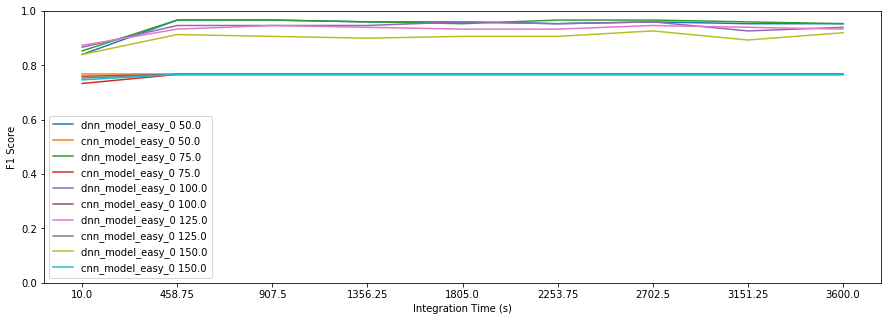
\includegraphics[width=\textwidth]{images/results_easy_distance_comparison}
         \caption{Simplified Dataset.}
         \label{fig:results_full_background_inject_simple}
     \end{subfigure}

     \begin{subfigure}[b]{0.9\textwidth}
         \centering
         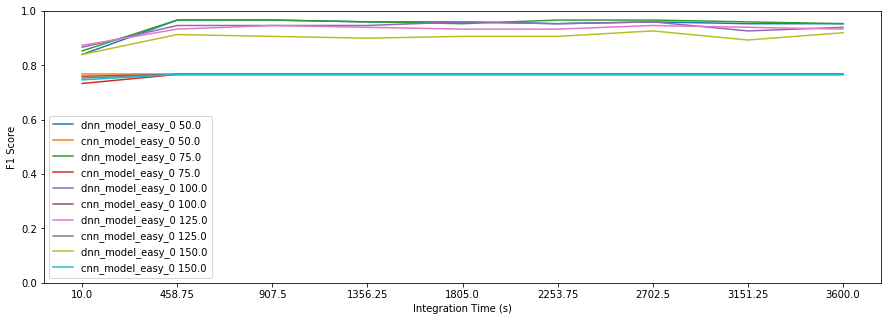
\includegraphics[width=\textwidth]{images/results_easy_distance_comparison}
         \caption{Complete Dataset.}
         \label{fig:results_full_background_inject_full}
     \end{subfigure}

        \caption{F1 score for models tested on ANSI isotope combinations.}
        \label{fig:results_full_background_inject}
\end{figure}



\subsection{Results on Measured Spectra}

This section shows model asymptotic performance vs integration time for a few different settings (different voltages, shielding)

To investigate how each model identified real spectra behind shielding and spectra with different calibrations, real spectra were measured. Sources include $^{137}$Cs, $^{60}$Co, $^{133}$Ba, and $^{152}$Eu. 


\subsubsection{Asymptotic Model Performance on Changing Voltage}

To see the generalization performance of the model to changing calibration, spectra with different voltages are recorded and their asymptotic performance compared.

Spectra were measured with different detector calibrations. A 2x2 Ortec NaI detector was set to 770 V, setting it's 1024th channel to 3 MeV. To capture a large range of calibrations, voltages varied from 720 V to 820 V in steps of 15 V. The $^{137}$Cs, $^{60}$Co, and $^{133}$Ba source had an activity of 1$\mu$C. For these sources, a source-to-detector distance of 14.25 mm was used to keep the cps on the detector from the source equal to the cps on the detector from background.

Figures \ref{fig:model_asymptotic_performance_co60} and \ref{fig:model_asymptotic_performance_cs137} show performance for isotopes with comparatively simplified spectra.


\begin{figure}[H]
     \centering
     \begin{subfigure}[b]{0.9\textwidth}
         \centering
         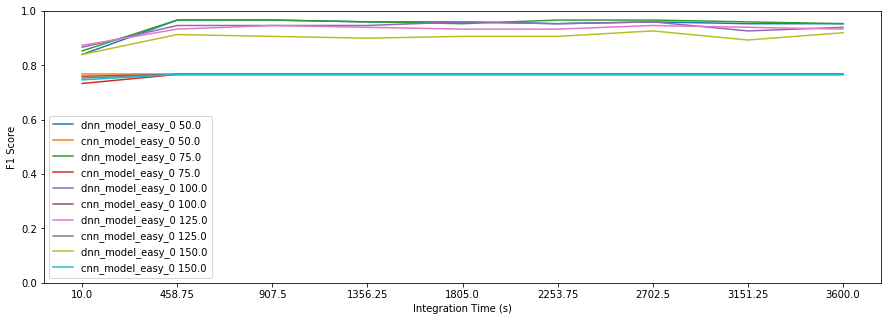
\includegraphics[width=\textwidth]{images/results_easy_distance_comparison}
         \caption{$^{60}$Co}
         \label{fig:model_asymptotic_performance_co60}
     \end{subfigure}

     \begin{subfigure}[b]{0.9\textwidth}
         \centering
         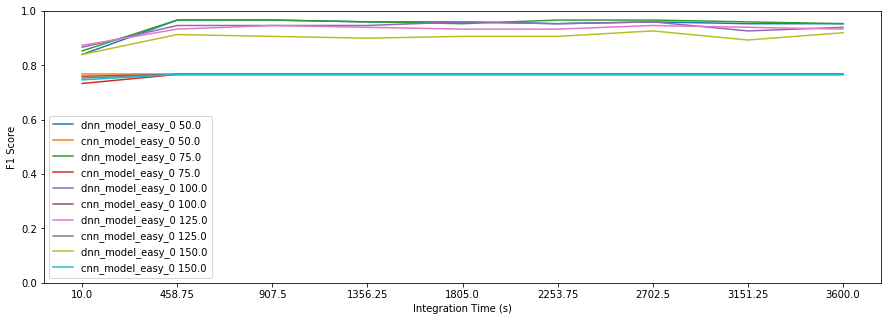
\includegraphics[width=\textwidth]{images/results_easy_distance_comparison}
         \caption{$^{137}$Cs.}
         \label{fig:results_easy_distance_comparison_full}
     \end{subfigure}
     
     \begin{subfigure}[b]{0.9\textwidth}
         \centering
         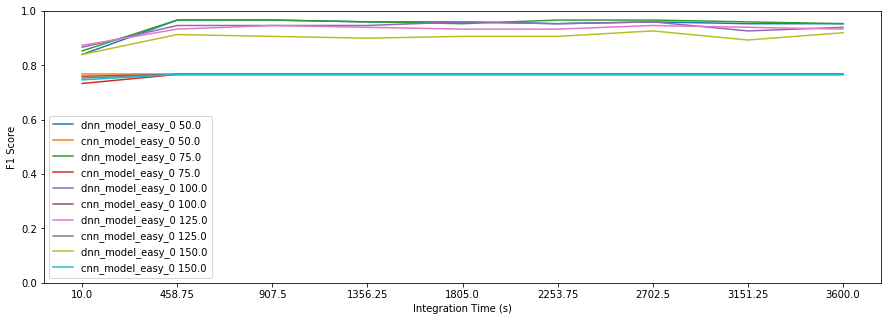
\includegraphics[width=\textwidth]{images/results_easy_distance_comparison}
         \caption{$^{152}$Eu.}
         \label{fig:results_easy_distance_comparison_full}
     \end{subfigure}
     
     \begin{subfigure}[b]{0.9\textwidth}
         \centering
         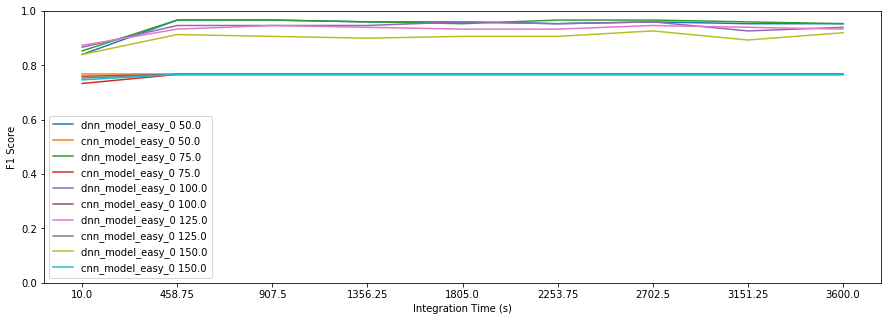
\includegraphics[width=\textwidth]{images/results_easy_distance_comparison}
         \caption{$^{133}$Ba.}
         \label{fig:results_easy_distance_comparison_full}
     \end{subfigure}

        \caption{F1 score for all models trained on the simplified dataset. Spectra measured with different gain settings.}
        \label{fig:results_easy_distance_comparison}
\end{figure}


\begin{figure}[H]
     \centering
     \begin{subfigure}[b]{0.9\textwidth}
         \centering
         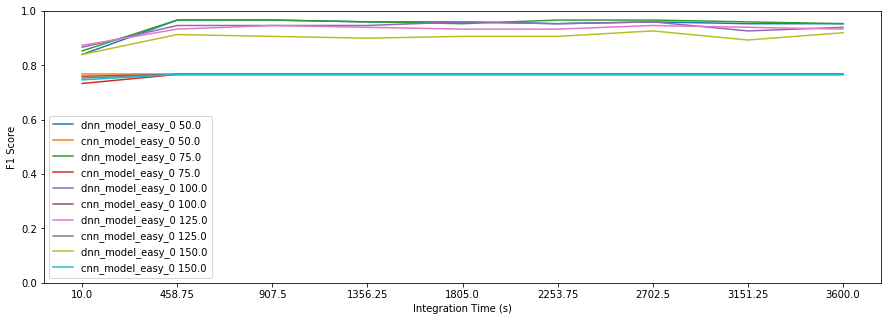
\includegraphics[width=\textwidth]{images/results_easy_distance_comparison}
         \caption{$^{60}$Co}
         \label{fig:model_asymptotic_performance_co60}
     \end{subfigure}

     \begin{subfigure}[b]{0.9\textwidth}
         \centering
         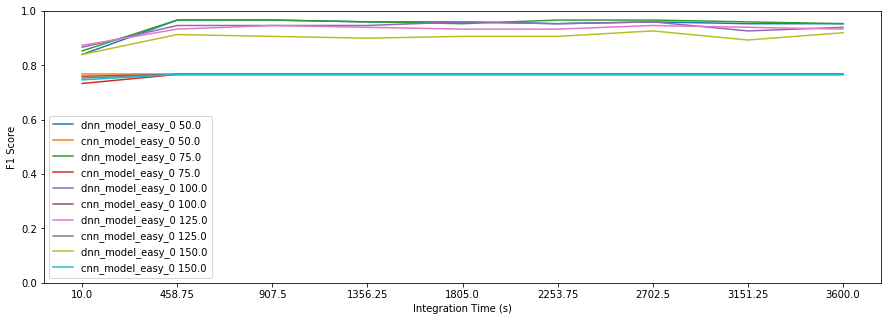
\includegraphics[width=\textwidth]{images/results_easy_distance_comparison}
         \caption{$^{137}$Cs.}
         \label{fig:results_easy_distance_comparison_full}
     \end{subfigure}
     
     \begin{subfigure}[b]{0.9\textwidth}
         \centering
         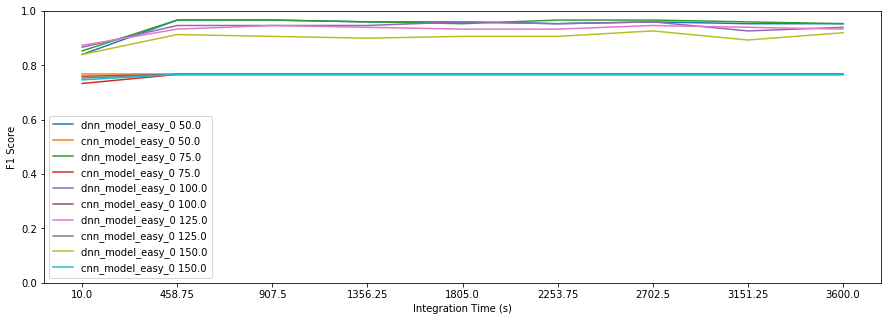
\includegraphics[width=\textwidth]{images/results_easy_distance_comparison}
         \caption{$^{152}$Eu.}
         \label{fig:results_easy_distance_comparison_full}
     \end{subfigure}
     
     \begin{subfigure}[b]{0.9\textwidth}
         \centering
         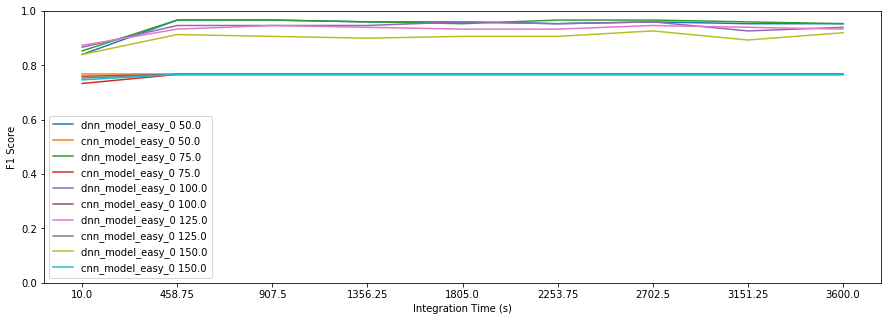
\includegraphics[width=\textwidth]{images/results_easy_distance_comparison}
         \caption{$^{133}$Ba.}
         \label{fig:results_easy_distance_comparison_full}
     \end{subfigure}

        \caption{F1 score for all models trained on the complete dataset. Spectra measured with different gain settings.}
        \label{fig:results_easy_distance_comparison}
\end{figure}


